\addchap{Was ist das hier?}


Hallo! Bis hierher hast du es nun schon mal geschafft. Wahnsinn!

Wie du vielleicht im Verlauf deines jetzt beginnenden Studiums feststellen wirst, ist es eine der schwersten Aufgaben, einen Informatiker zum Lesen des Handbuchs oder der Dokumentation zu bewegen. Vielleicht ist das so ein Spleen, der uns anhängt, vielleicht basteln wir aber auch einfach lieber tagelang an einem Problem, als eine halbe Stunde zum Nachschlagen im Handbuch zu investieren.
Oft wird euch deshalb in Foren oder bei StackOverflow der Satz entgegenschlagen: \enquote{RTFM} -- Read the fucking manual.

Aber die gute Nachricht ist, wenn ihr das hier lest, tretet ihr diesem Vorurteil schon mal entgegen. Denn dieses Heft ist ein kleines Handbuch für euer Studium.
Es verrät euch, wie die Uni funktioniert, Lehrveranstaltungen aufgebaut sind, ihr euch in Prüfungen einschreibt, was der Campus alles zu bieten hat und noch vieles mehr.
Wie jedes gute Handbuch enthält es dabei viel zu viele Informationen, die man kaum auf einmal brauchen oder verarbeiten kann.

Deswegen reicht es auch, wenn ihr euch jetzt beim Lesen auf alle mit \keys{must read} gekennzeichneten Kapitel beschränkt und den Rest später mal nachschlagt oder euch über die FAQ-Sektion auf Seite~\pageref{sec:faq} zu den passenden Antworten durchhangelt.
Dieses Buch ist so angelegt, dass es euch über den Großteil eures Studiums mit Informationen und Antworten weiterhelfen kann. Hebt es euch also auf und kramt es immer mal wieder raus. Wie jedes gute Handbuch :)

Und jetzt erstmal weg mit dem Schmöker! Dich erwartet die Erstsemestereinführung (ESE), die dir in der kommenden Woche erstmal das Wichtigste erklärt.
Genieß diese Zeit und mach dich bereit für die noch spannendere, die dich jetzt erwartet!

\textbf{Bleibt nur noch zu sagen: Viel Spaß in der ESE und im Studium!}

% \begin{figure}[b!]
% 	\centering
% 	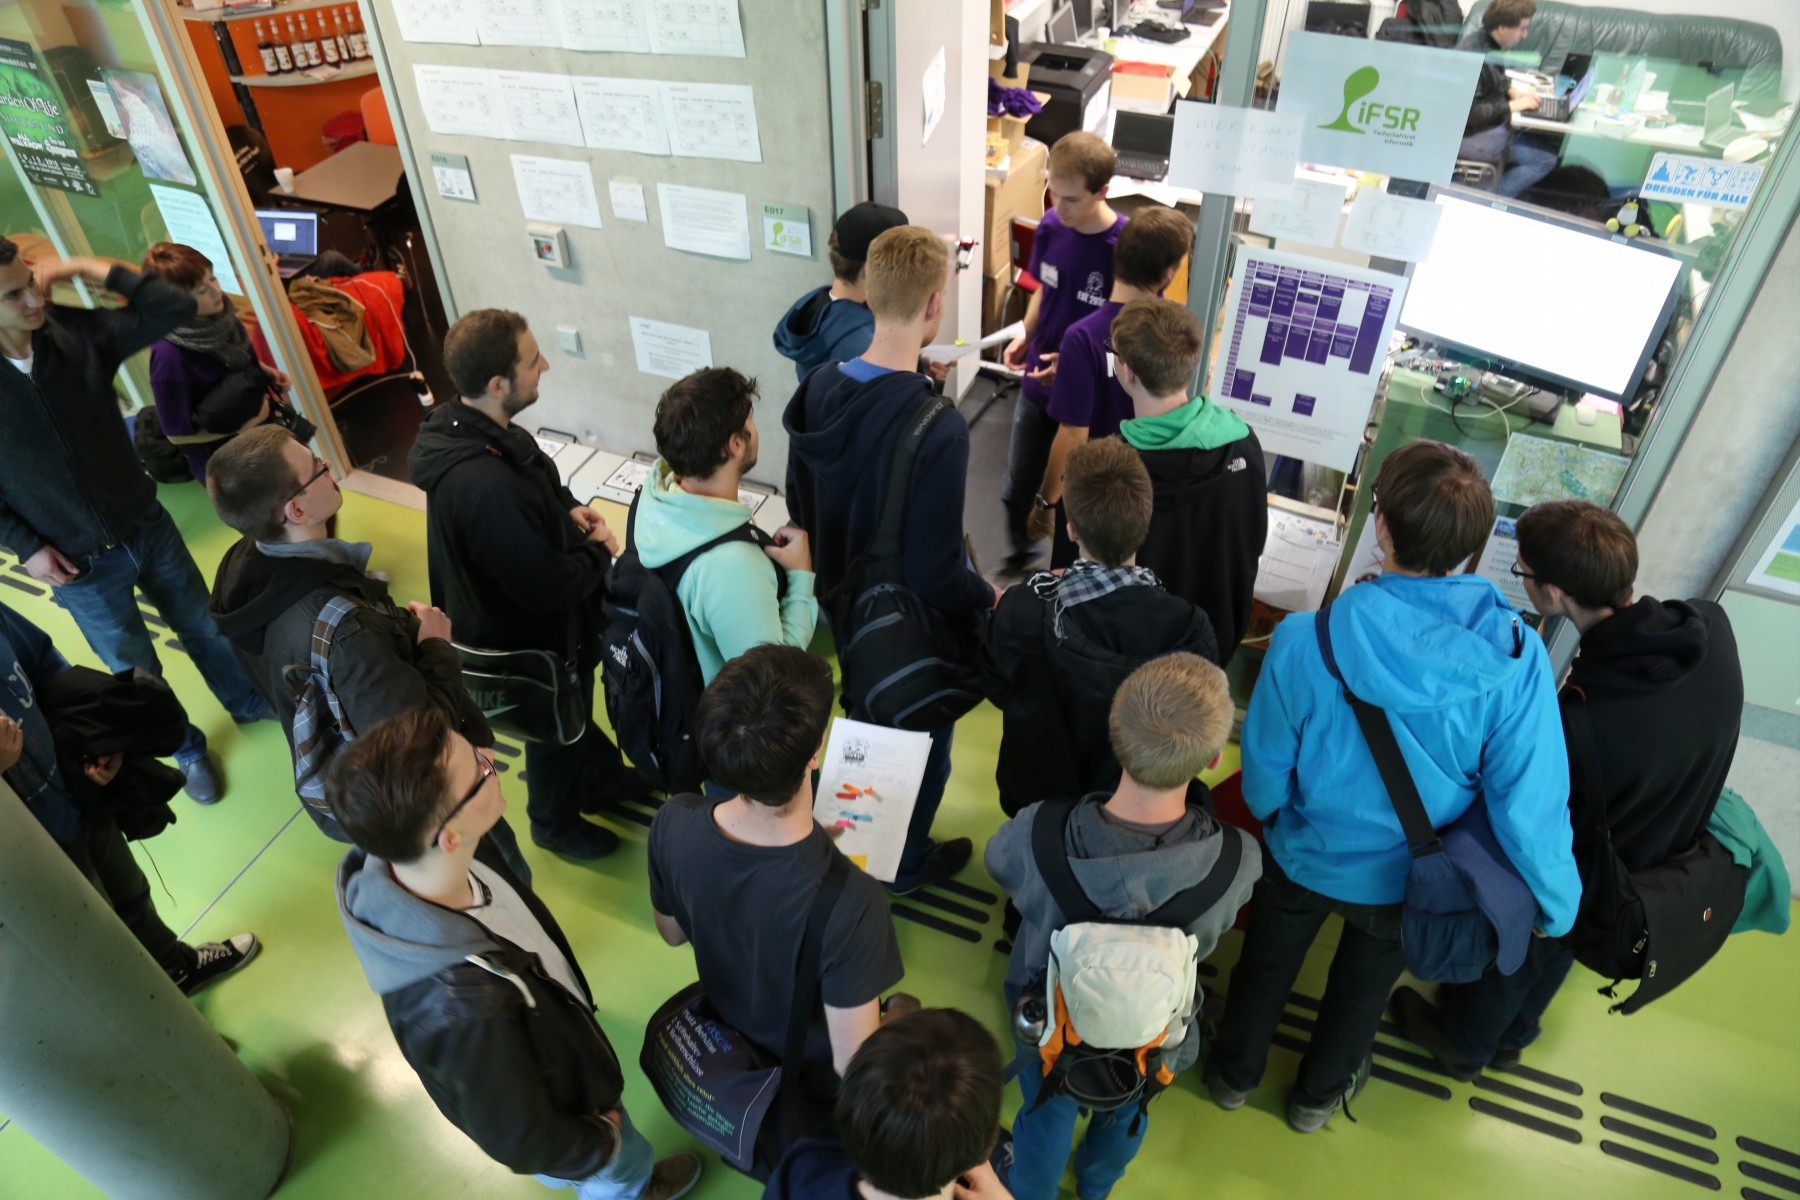
\includegraphics[trim={0 5.5cm 0 0}, clip, width=\linewidth]{img/ese2015/bueroansturm.jpg}
% \end{figure}%

\begin{awesomeblock}[ese_bg_color]{2pt}{\faLightbulb[regular]}{ese_bg_color}
    \begin{minipage}[t]{.82\textwidth}
\small PS\@: Links schauen in diesem Heft so aus: \link{https://html5zombo.com}. Ganz hinten auf einer der letzten Seiten kannst du dann die Adresse nachsehen. Ebenfalls kannst du auch direkt unter \url{ese.ifsr.de/2021/<Zahl>} auf die verlinkte Seite weitergeleitet werden.
    \end{minipage}
\end{awesomeblock}
